\documentclass[xcolor=dvipsnames,table]{beamer}

\usepackage{latexsym}
\usepackage[utf8]{inputenc}
\usepackage[brazil]{babel}
\usepackage{amssymb}
\usepackage{amsmath}
\usepackage{stmaryrd}
\usepackage{fancybox}
\usepackage{datetime}
\usepackage[T1]{fontenc}
\usepackage{graphicx}
\usepackage{graphics}
\usepackage{url}
\usepackage{algorithmic}
\usepackage{algorithm}
\usepackage{acronym}
\usepackage{array}

\newtheorem{definicao}{Definio}
\newcommand{\tab}{\hspace*{2em}}

\mode<presentation>
{
  \definecolor{colortexto}{RGB}{0,0,0}
 
  \setbeamertemplate{background canvas}[vertical shading][ bottom=white!10,top=white!10]
  \setbeamercolor{normal text}{fg=colortexto} 

  \usetheme{Warsaw}
}

\title{Máquina de Turing} 

\author{
  Esdras Lins Bispo Jr. \\ \url{bispojr@ufg.br}
  } 
 \institute{
  Teoria da Computação \\Bacharelado em Ciência da Computação}
\date{\textbf{15 de maio de 2017} }

\logo{
\includegraphics[width=1cm]{images/ufgJataiLogo.png}}

\begin{document}

	\begin{frame}
		\titlepage
	\end{frame}

	\AtBeginSection{
		\begin{frame}{Sumário}%[allowframebreaks]{Sumário}
    		\tableofcontents[currentsection]
    		%\tableofcontents[currentsection, hideothersubsections]
		\end{frame}
	}

	\begin{frame}{Plano de Aula}
		\tableofcontents
		%\tableofcontents[hideallsubsections]
	\end{frame}

%------------------------------------------
	\begin{frame}{Bônus (0,5 pt)}
		\begin{block}{Desafio}
			\begin{itemize}
				\item {\bf Problema 2.30 (a):} Mostre que a linguagem $C =  \{0^n 1^n 0^n 1^n \mbox{ | } n \geq 0\}$ não é livre-de-contexto. 
				\item Candidaturas agora; 
				\item Apresentação e resposta por escrito $\rightarrow$ \\segunda (22 de maio, 17h10); 
				\item 10 minutos de apresentação.
			\end{itemize}
		\end{block} 
		\begin{block}{Livro}
			SIPSER, M. {\bf Introdução à Teoria da Computação}, 2a Edição, Editora Thomson Learning, 2011. \color{blue}{\bf Código Bib.: [004 SIP/int]}.
		\end{block}
	\end{frame}
    
    \section{Revisão}
	\subsection{Máquina de Turing}
	\begin{frame}{Configuração de uma MT}
		A configuração $C_1$ {\bf origina} a configuração $C_2$, se a máquina de Turing puder legitimamente ir de $C_1$ para $C_2$. 
		\begin{block}{Mais formalmente...}					Para:
			\begin{itemize}
				\item {\tt a, b, c} $\in \Gamma$, 
				\item {\tt u, v} $\in \Gamma^*$,  
				\item os estados $q_i$ e $q_j$, 
				\item as configurações {\tt ua}$q_i${\tt bv} e {\tt u}$q_j${\tt acv}. 
				\end{itemize}
			Digamos que 
			\begin{center}
				{\tt ua}$q_i${\tt bv} origina {\tt u}$q_j${\tt acv} 
			\end{center} 
			se na função de transição $\delta(q_i, b) = (q_j, c, E)$.
		\end{block}
	\end{frame}
	
	\begin{frame}{Configuração de uma MT}
		\begin{block}{Mais formalmente...}
			Digamos que 
			\begin{center}
				{\tt ua}$q_i${\tt bv} origina {\tt u}$q_j${\tt acv} 
			\end{center} 
			se na função de transição $\delta(q_i, b) = (q_j, c, E)$. Ou
			\begin{center}
				{\tt ua}$q_i${\tt bv} origina {\tt uac}$q_j${\tt v} 
			\end{center} 
			se na função de transição $\delta(q_i, b) = (q_j, c, D)$.
		\end{block}
	\end{frame}
	
	\begin{frame}{Linguagem de uma MT}
		Uma máquina de Turing $M$ {\bf aceita} a entrada $\omega$ se uma sequência de configurações $C_1, C_2, \ldots, C_k$ existe, de forma que 
		\begin{itemize}
			\item $C_1$ é a configuração inicial de $M$ sobre a entrada $\omega$;
			\item cada $C_i$ origina $C_{i+1}$;
			\item $C_k$ é uma configuração de aceitação.
		\end{itemize} 
		
		\begin{block}{Linguagem de $M$}
			É a coleção de cadeias que $M$ aceita. Também chamada de {\bf linguagem reconhecida por $M$} e denotada por $L(M)$.
		\end{block}		
	\end{frame}

	 \begin{frame}{Definições}
		\begin{block}{Definição}
			Chame uma linguagem de {\bf Turing-reconhecível}, se alguma máquina de Turing a reconhece.
		\end{block}
		\begin{block}{Definição}
			Chame uma linguagem de {\bf Turing-decidível}, se alguma máquina de Turing a decide.
		\end{block}
		\begin{block}{Corolário}
			Toda linguagem Turing-decidível é Turing-reconhecível.
		\end{block}
	\end{frame}		
	
	\begin{frame}{Exemplos}
		Uma máquina de Turing $M_2$ que decide $A = \{ 0^{2^n} \mbox{ | } n \geq 0 \}$: 
		\begin{center}
			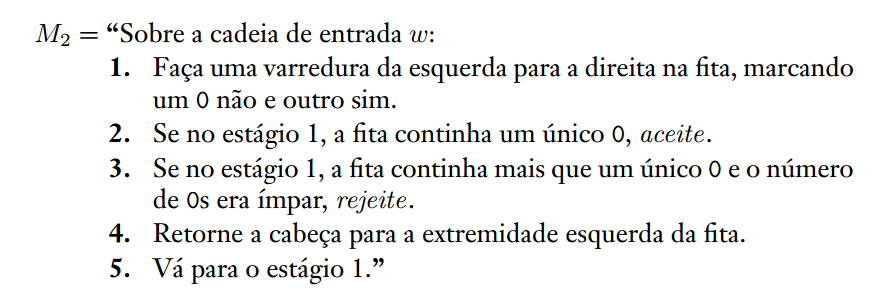
\includegraphics[height=3.5cm]{images/m2.png}
		\end{center}
	\end{frame}
	
	\begin{frame}{Exemplos}
		\begin{block}{Descrição Formal de $M_2$}
			$M_2 = (Q, \Sigma, \Gamma, \delta, q_1, q_{aceita}, q_{rejeita})$:
			\begin{itemize}
				\item $Q = \{ q_1, q_2, q_3, q_4, q_5, q_{aceita}, q_{rejeita} \}$;
				\item $\Sigma = \{ 0 \}$,
				\item $\Gamma = \{ 0, x, \sqcup \}$,
				\item Descrevemos $\delta$ no próximo slide; e
				\item $q_1, q_{aceita}$ e $q_{rejeita}$ são o estado inicial, de aceitação e de rejeição, respectivamente.
			\end{itemize}
		\end{block}
	\end{frame}
	
	\begin{frame}{Exemplos}
		\begin{center}
			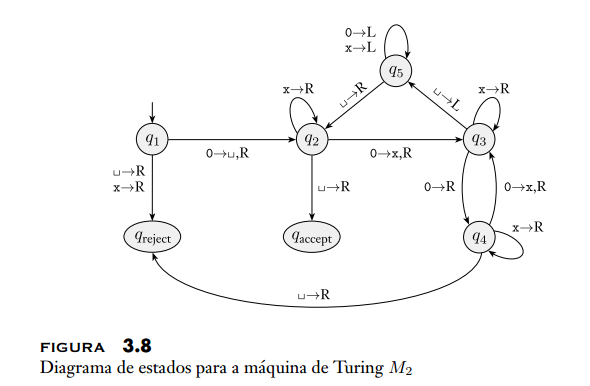
\includegraphics[height=7cm]{images/fig38.png}
		\end{center}
	\end{frame}
	
	\section{Máquina de Turing}
	\begin{frame}{Problema}
		\begin{block}{Problema 3.15 (a)}
			Mostre que a coleção de linguagens decidíveis é fechada sob a operação de união.		
		\end{block} \pause
		\begin{center}
			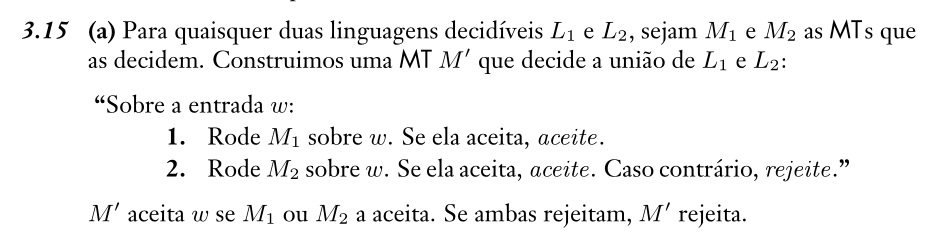
\includegraphics[height=2.7cm]{images/ex3-15a}
		\end{center}
	\end{frame}
	
	\section{Variantes da MT}
	\subsection{MT Multifita}
	\begin{frame}[shrink]{MT Multifita}
		\begin{block}{Definição}
			Uma {\bf máquina de Turing multifita} é como uma máquina de Turing comum com várias fitas:
			\begin{itemize} \pause
				\item cada fita tem sua própria cabeça de leitura e escrita; \pause
				\item a configuração inicial consiste da cadeia de entrada aparecer sobre a fita 1, e as outras iniciar em branco; \pause
				\item a função de transição permite ler, escrever e mover as cabeças em algumas ou em todas as fitas simultaneamente
				\begin{center}
					$\delta : Q \times \Gamma^k \rightarrow Q \times \Gamma^k \times \{E,D,P\}^k$
				\end{center}
				em que $k$ é o número de fitas.
			\end{itemize}
		\end{block}\pause
		\begin{block}{Exemplo}
			$\delta(q_i, a_1, \ldots, a_k) = (q_j, b_1, \ldots, b_k, P, D, \ldots, E)$
		\end{block}
	\end{frame}
	
	\begin{frame}{MT Multifita}
		\begin{block}{Teorema}
			Toda máquina de Turing multifita tem uma máquina de Turing de uma única fita que lhe é equivalente.
		\end{block}
	\end{frame}
	
	\begin{frame}{MT Multifita}
		\begin{center}
			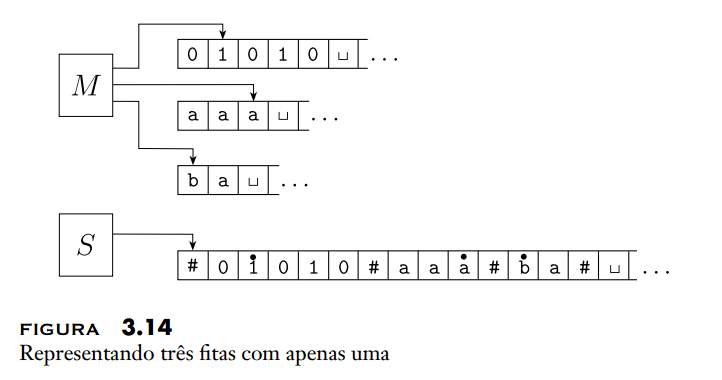
\includegraphics[height=6cm]{images/fig314.png}
		\end{center}
	\end{frame}
	
	\begin{frame}{MT Multifita}
		\begin{center}
			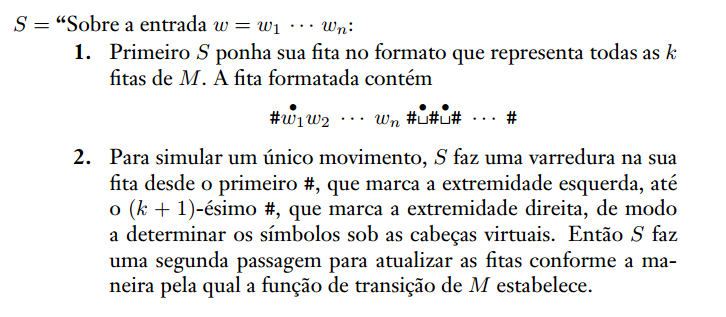
\includegraphics[height=5cm]{images/teoMt-1.png}
		\end{center}
	\end{frame}
	
	\begin{frame}{MT Multifita}
		\begin{center}
			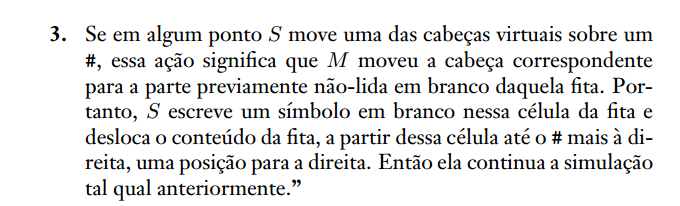
\includegraphics[height=3.3cm]{images/teoMt-2.png}
		\end{center}
	\end{frame}
	
	\begin{frame}{MT Multifita}
		\begin{block}{Teorema}
			Toda máquina de Turing multifita tem uma máquina de Turing de uma única fita que lhe é equivalente.
		\end{block} \pause
		\begin{block}{Corolário}
			Uma linguagem é Turing-reconhecível se e somente se alguma máquina de Turing multifita a reconhece.
		\end{block}
	\end{frame}
	
	\begin{frame}{MT Multifita}
		\begin{center}
			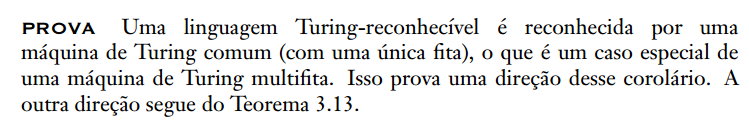
\includegraphics[height=1.8cm]{images/provaCorolario.png}
		\end{center}
	\end{frame}
	
	\begin{frame}
		\titlepage
	\end{frame}
	
\end{document}